
% Default to the notebook output style

    


% Inherit from the specified cell style.




    
\documentclass[11pt]{article}

    
    
    \usepackage[T1]{fontenc}
    % Nicer default font (+ math font) than Computer Modern for most use cases
    \usepackage{mathpazo}

    % Basic figure setup, for now with no caption control since it's done
    % automatically by Pandoc (which extracts ![](path) syntax from Markdown).
    \usepackage{graphicx}
    % We will generate all images so they have a width \maxwidth. This means
    % that they will get their normal width if they fit onto the page, but
    % are scaled down if they would overflow the margins.
    \makeatletter
    \def\maxwidth{\ifdim\Gin@nat@width>\linewidth\linewidth
    \else\Gin@nat@width\fi}
    \makeatother
    \let\Oldincludegraphics\includegraphics
    % Set max figure width to be 80% of text width, for now hardcoded.
    \renewcommand{\includegraphics}[1]{\Oldincludegraphics[width=.8\maxwidth]{#1}}
    % Ensure that by default, figures have no caption (until we provide a
    % proper Figure object with a Caption API and a way to capture that
    % in the conversion process - todo).
    \usepackage{caption}
    \DeclareCaptionLabelFormat{nolabel}{}
    \captionsetup{labelformat=nolabel}

    \usepackage{adjustbox} % Used to constrain images to a maximum size 
    \usepackage{xcolor} % Allow colors to be defined
    \usepackage{enumerate} % Needed for markdown enumerations to work
    \usepackage{geometry} % Used to adjust the document margins
    \usepackage{amsmath} % Equations
    \usepackage{amssymb} % Equations
    \usepackage{textcomp} % defines textquotesingle
    % Hack from http://tex.stackexchange.com/a/47451/13684:
    \AtBeginDocument{%
        \def\PYZsq{\textquotesingle}% Upright quotes in Pygmentized code
    }
    \usepackage{upquote} % Upright quotes for verbatim code
    \usepackage{eurosym} % defines \euro
    \usepackage[mathletters]{ucs} % Extended unicode (utf-8) support
    \usepackage[utf8x]{inputenc} % Allow utf-8 characters in the tex document
    \usepackage{fancyvrb} % verbatim replacement that allows latex
    \usepackage{grffile} % extends the file name processing of package graphics 
                         % to support a larger range 
    % The hyperref package gives us a pdf with properly built
    % internal navigation ('pdf bookmarks' for the table of contents,
    % internal cross-reference links, web links for URLs, etc.)
    \usepackage{hyperref}
    \usepackage{longtable} % longtable support required by pandoc >1.10
    \usepackage{booktabs}  % table support for pandoc > 1.12.2
    \usepackage[inline]{enumitem} % IRkernel/repr support (it uses the enumerate* environment)
    \usepackage[normalem]{ulem} % ulem is needed to support strikethroughs (\sout)
                                % normalem makes italics be italics, not underlines
    

    
    
    % Colors for the hyperref package
    \definecolor{urlcolor}{rgb}{0,.145,.698}
    \definecolor{linkcolor}{rgb}{.71,0.21,0.01}
    \definecolor{citecolor}{rgb}{.12,.54,.11}

    % ANSI colors
    \definecolor{ansi-black}{HTML}{3E424D}
    \definecolor{ansi-black-intense}{HTML}{282C36}
    \definecolor{ansi-red}{HTML}{E75C58}
    \definecolor{ansi-red-intense}{HTML}{B22B31}
    \definecolor{ansi-green}{HTML}{00A250}
    \definecolor{ansi-green-intense}{HTML}{007427}
    \definecolor{ansi-yellow}{HTML}{DDB62B}
    \definecolor{ansi-yellow-intense}{HTML}{B27D12}
    \definecolor{ansi-blue}{HTML}{208FFB}
    \definecolor{ansi-blue-intense}{HTML}{0065CA}
    \definecolor{ansi-magenta}{HTML}{D160C4}
    \definecolor{ansi-magenta-intense}{HTML}{A03196}
    \definecolor{ansi-cyan}{HTML}{60C6C8}
    \definecolor{ansi-cyan-intense}{HTML}{258F8F}
    \definecolor{ansi-white}{HTML}{C5C1B4}
    \definecolor{ansi-white-intense}{HTML}{A1A6B2}

    % commands and environments needed by pandoc snippets
    % extracted from the output of `pandoc -s`
    \providecommand{\tightlist}{%
      \setlength{\itemsep}{0pt}\setlength{\parskip}{0pt}}
    \DefineVerbatimEnvironment{Highlighting}{Verbatim}{commandchars=\\\{\}}
    % Add ',fontsize=\small' for more characters per line
    \newenvironment{Shaded}{}{}
    \newcommand{\KeywordTok}[1]{\textcolor[rgb]{0.00,0.44,0.13}{\textbf{{#1}}}}
    \newcommand{\DataTypeTok}[1]{\textcolor[rgb]{0.56,0.13,0.00}{{#1}}}
    \newcommand{\DecValTok}[1]{\textcolor[rgb]{0.25,0.63,0.44}{{#1}}}
    \newcommand{\BaseNTok}[1]{\textcolor[rgb]{0.25,0.63,0.44}{{#1}}}
    \newcommand{\FloatTok}[1]{\textcolor[rgb]{0.25,0.63,0.44}{{#1}}}
    \newcommand{\CharTok}[1]{\textcolor[rgb]{0.25,0.44,0.63}{{#1}}}
    \newcommand{\StringTok}[1]{\textcolor[rgb]{0.25,0.44,0.63}{{#1}}}
    \newcommand{\CommentTok}[1]{\textcolor[rgb]{0.38,0.63,0.69}{\textit{{#1}}}}
    \newcommand{\OtherTok}[1]{\textcolor[rgb]{0.00,0.44,0.13}{{#1}}}
    \newcommand{\AlertTok}[1]{\textcolor[rgb]{1.00,0.00,0.00}{\textbf{{#1}}}}
    \newcommand{\FunctionTok}[1]{\textcolor[rgb]{0.02,0.16,0.49}{{#1}}}
    \newcommand{\RegionMarkerTok}[1]{{#1}}
    \newcommand{\ErrorTok}[1]{\textcolor[rgb]{1.00,0.00,0.00}{\textbf{{#1}}}}
    \newcommand{\NormalTok}[1]{{#1}}
    
    % Additional commands for more recent versions of Pandoc
    \newcommand{\ConstantTok}[1]{\textcolor[rgb]{0.53,0.00,0.00}{{#1}}}
    \newcommand{\SpecialCharTok}[1]{\textcolor[rgb]{0.25,0.44,0.63}{{#1}}}
    \newcommand{\VerbatimStringTok}[1]{\textcolor[rgb]{0.25,0.44,0.63}{{#1}}}
    \newcommand{\SpecialStringTok}[1]{\textcolor[rgb]{0.73,0.40,0.53}{{#1}}}
    \newcommand{\ImportTok}[1]{{#1}}
    \newcommand{\DocumentationTok}[1]{\textcolor[rgb]{0.73,0.13,0.13}{\textit{{#1}}}}
    \newcommand{\AnnotationTok}[1]{\textcolor[rgb]{0.38,0.63,0.69}{\textbf{\textit{{#1}}}}}
    \newcommand{\CommentVarTok}[1]{\textcolor[rgb]{0.38,0.63,0.69}{\textbf{\textit{{#1}}}}}
    \newcommand{\VariableTok}[1]{\textcolor[rgb]{0.10,0.09,0.49}{{#1}}}
    \newcommand{\ControlFlowTok}[1]{\textcolor[rgb]{0.00,0.44,0.13}{\textbf{{#1}}}}
    \newcommand{\OperatorTok}[1]{\textcolor[rgb]{0.40,0.40,0.40}{{#1}}}
    \newcommand{\BuiltInTok}[1]{{#1}}
    \newcommand{\ExtensionTok}[1]{{#1}}
    \newcommand{\PreprocessorTok}[1]{\textcolor[rgb]{0.74,0.48,0.00}{{#1}}}
    \newcommand{\AttributeTok}[1]{\textcolor[rgb]{0.49,0.56,0.16}{{#1}}}
    \newcommand{\InformationTok}[1]{\textcolor[rgb]{0.38,0.63,0.69}{\textbf{\textit{{#1}}}}}
    \newcommand{\WarningTok}[1]{\textcolor[rgb]{0.38,0.63,0.69}{\textbf{\textit{{#1}}}}}
    
    
    % Define a nice break command that doesn't care if a line doesn't already
    % exist.
    \def\br{\hspace*{\fill} \\* }
    % Math Jax compatability definitions
    \def\gt{>}
    \def\lt{<}
    % Document parameters
    \title{Assignment-2}
    
    
    

    % Pygments definitions
    
\makeatletter
\def\PY@reset{\let\PY@it=\relax \let\PY@bf=\relax%
    \let\PY@ul=\relax \let\PY@tc=\relax%
    \let\PY@bc=\relax \let\PY@ff=\relax}
\def\PY@tok#1{\csname PY@tok@#1\endcsname}
\def\PY@toks#1+{\ifx\relax#1\empty\else%
    \PY@tok{#1}\expandafter\PY@toks\fi}
\def\PY@do#1{\PY@bc{\PY@tc{\PY@ul{%
    \PY@it{\PY@bf{\PY@ff{#1}}}}}}}
\def\PY#1#2{\PY@reset\PY@toks#1+\relax+\PY@do{#2}}

\expandafter\def\csname PY@tok@w\endcsname{\def\PY@tc##1{\textcolor[rgb]{0.73,0.73,0.73}{##1}}}
\expandafter\def\csname PY@tok@c\endcsname{\let\PY@it=\textit\def\PY@tc##1{\textcolor[rgb]{0.25,0.50,0.50}{##1}}}
\expandafter\def\csname PY@tok@cp\endcsname{\def\PY@tc##1{\textcolor[rgb]{0.74,0.48,0.00}{##1}}}
\expandafter\def\csname PY@tok@k\endcsname{\let\PY@bf=\textbf\def\PY@tc##1{\textcolor[rgb]{0.00,0.50,0.00}{##1}}}
\expandafter\def\csname PY@tok@kp\endcsname{\def\PY@tc##1{\textcolor[rgb]{0.00,0.50,0.00}{##1}}}
\expandafter\def\csname PY@tok@kt\endcsname{\def\PY@tc##1{\textcolor[rgb]{0.69,0.00,0.25}{##1}}}
\expandafter\def\csname PY@tok@o\endcsname{\def\PY@tc##1{\textcolor[rgb]{0.40,0.40,0.40}{##1}}}
\expandafter\def\csname PY@tok@ow\endcsname{\let\PY@bf=\textbf\def\PY@tc##1{\textcolor[rgb]{0.67,0.13,1.00}{##1}}}
\expandafter\def\csname PY@tok@nb\endcsname{\def\PY@tc##1{\textcolor[rgb]{0.00,0.50,0.00}{##1}}}
\expandafter\def\csname PY@tok@nf\endcsname{\def\PY@tc##1{\textcolor[rgb]{0.00,0.00,1.00}{##1}}}
\expandafter\def\csname PY@tok@nc\endcsname{\let\PY@bf=\textbf\def\PY@tc##1{\textcolor[rgb]{0.00,0.00,1.00}{##1}}}
\expandafter\def\csname PY@tok@nn\endcsname{\let\PY@bf=\textbf\def\PY@tc##1{\textcolor[rgb]{0.00,0.00,1.00}{##1}}}
\expandafter\def\csname PY@tok@ne\endcsname{\let\PY@bf=\textbf\def\PY@tc##1{\textcolor[rgb]{0.82,0.25,0.23}{##1}}}
\expandafter\def\csname PY@tok@nv\endcsname{\def\PY@tc##1{\textcolor[rgb]{0.10,0.09,0.49}{##1}}}
\expandafter\def\csname PY@tok@no\endcsname{\def\PY@tc##1{\textcolor[rgb]{0.53,0.00,0.00}{##1}}}
\expandafter\def\csname PY@tok@nl\endcsname{\def\PY@tc##1{\textcolor[rgb]{0.63,0.63,0.00}{##1}}}
\expandafter\def\csname PY@tok@ni\endcsname{\let\PY@bf=\textbf\def\PY@tc##1{\textcolor[rgb]{0.60,0.60,0.60}{##1}}}
\expandafter\def\csname PY@tok@na\endcsname{\def\PY@tc##1{\textcolor[rgb]{0.49,0.56,0.16}{##1}}}
\expandafter\def\csname PY@tok@nt\endcsname{\let\PY@bf=\textbf\def\PY@tc##1{\textcolor[rgb]{0.00,0.50,0.00}{##1}}}
\expandafter\def\csname PY@tok@nd\endcsname{\def\PY@tc##1{\textcolor[rgb]{0.67,0.13,1.00}{##1}}}
\expandafter\def\csname PY@tok@s\endcsname{\def\PY@tc##1{\textcolor[rgb]{0.73,0.13,0.13}{##1}}}
\expandafter\def\csname PY@tok@sd\endcsname{\let\PY@it=\textit\def\PY@tc##1{\textcolor[rgb]{0.73,0.13,0.13}{##1}}}
\expandafter\def\csname PY@tok@si\endcsname{\let\PY@bf=\textbf\def\PY@tc##1{\textcolor[rgb]{0.73,0.40,0.53}{##1}}}
\expandafter\def\csname PY@tok@se\endcsname{\let\PY@bf=\textbf\def\PY@tc##1{\textcolor[rgb]{0.73,0.40,0.13}{##1}}}
\expandafter\def\csname PY@tok@sr\endcsname{\def\PY@tc##1{\textcolor[rgb]{0.73,0.40,0.53}{##1}}}
\expandafter\def\csname PY@tok@ss\endcsname{\def\PY@tc##1{\textcolor[rgb]{0.10,0.09,0.49}{##1}}}
\expandafter\def\csname PY@tok@sx\endcsname{\def\PY@tc##1{\textcolor[rgb]{0.00,0.50,0.00}{##1}}}
\expandafter\def\csname PY@tok@m\endcsname{\def\PY@tc##1{\textcolor[rgb]{0.40,0.40,0.40}{##1}}}
\expandafter\def\csname PY@tok@gh\endcsname{\let\PY@bf=\textbf\def\PY@tc##1{\textcolor[rgb]{0.00,0.00,0.50}{##1}}}
\expandafter\def\csname PY@tok@gu\endcsname{\let\PY@bf=\textbf\def\PY@tc##1{\textcolor[rgb]{0.50,0.00,0.50}{##1}}}
\expandafter\def\csname PY@tok@gd\endcsname{\def\PY@tc##1{\textcolor[rgb]{0.63,0.00,0.00}{##1}}}
\expandafter\def\csname PY@tok@gi\endcsname{\def\PY@tc##1{\textcolor[rgb]{0.00,0.63,0.00}{##1}}}
\expandafter\def\csname PY@tok@gr\endcsname{\def\PY@tc##1{\textcolor[rgb]{1.00,0.00,0.00}{##1}}}
\expandafter\def\csname PY@tok@ge\endcsname{\let\PY@it=\textit}
\expandafter\def\csname PY@tok@gs\endcsname{\let\PY@bf=\textbf}
\expandafter\def\csname PY@tok@gp\endcsname{\let\PY@bf=\textbf\def\PY@tc##1{\textcolor[rgb]{0.00,0.00,0.50}{##1}}}
\expandafter\def\csname PY@tok@go\endcsname{\def\PY@tc##1{\textcolor[rgb]{0.53,0.53,0.53}{##1}}}
\expandafter\def\csname PY@tok@gt\endcsname{\def\PY@tc##1{\textcolor[rgb]{0.00,0.27,0.87}{##1}}}
\expandafter\def\csname PY@tok@err\endcsname{\def\PY@bc##1{\setlength{\fboxsep}{0pt}\fcolorbox[rgb]{1.00,0.00,0.00}{1,1,1}{\strut ##1}}}
\expandafter\def\csname PY@tok@kc\endcsname{\let\PY@bf=\textbf\def\PY@tc##1{\textcolor[rgb]{0.00,0.50,0.00}{##1}}}
\expandafter\def\csname PY@tok@kd\endcsname{\let\PY@bf=\textbf\def\PY@tc##1{\textcolor[rgb]{0.00,0.50,0.00}{##1}}}
\expandafter\def\csname PY@tok@kn\endcsname{\let\PY@bf=\textbf\def\PY@tc##1{\textcolor[rgb]{0.00,0.50,0.00}{##1}}}
\expandafter\def\csname PY@tok@kr\endcsname{\let\PY@bf=\textbf\def\PY@tc##1{\textcolor[rgb]{0.00,0.50,0.00}{##1}}}
\expandafter\def\csname PY@tok@bp\endcsname{\def\PY@tc##1{\textcolor[rgb]{0.00,0.50,0.00}{##1}}}
\expandafter\def\csname PY@tok@fm\endcsname{\def\PY@tc##1{\textcolor[rgb]{0.00,0.00,1.00}{##1}}}
\expandafter\def\csname PY@tok@vc\endcsname{\def\PY@tc##1{\textcolor[rgb]{0.10,0.09,0.49}{##1}}}
\expandafter\def\csname PY@tok@vg\endcsname{\def\PY@tc##1{\textcolor[rgb]{0.10,0.09,0.49}{##1}}}
\expandafter\def\csname PY@tok@vi\endcsname{\def\PY@tc##1{\textcolor[rgb]{0.10,0.09,0.49}{##1}}}
\expandafter\def\csname PY@tok@vm\endcsname{\def\PY@tc##1{\textcolor[rgb]{0.10,0.09,0.49}{##1}}}
\expandafter\def\csname PY@tok@sa\endcsname{\def\PY@tc##1{\textcolor[rgb]{0.73,0.13,0.13}{##1}}}
\expandafter\def\csname PY@tok@sb\endcsname{\def\PY@tc##1{\textcolor[rgb]{0.73,0.13,0.13}{##1}}}
\expandafter\def\csname PY@tok@sc\endcsname{\def\PY@tc##1{\textcolor[rgb]{0.73,0.13,0.13}{##1}}}
\expandafter\def\csname PY@tok@dl\endcsname{\def\PY@tc##1{\textcolor[rgb]{0.73,0.13,0.13}{##1}}}
\expandafter\def\csname PY@tok@s2\endcsname{\def\PY@tc##1{\textcolor[rgb]{0.73,0.13,0.13}{##1}}}
\expandafter\def\csname PY@tok@sh\endcsname{\def\PY@tc##1{\textcolor[rgb]{0.73,0.13,0.13}{##1}}}
\expandafter\def\csname PY@tok@s1\endcsname{\def\PY@tc##1{\textcolor[rgb]{0.73,0.13,0.13}{##1}}}
\expandafter\def\csname PY@tok@mb\endcsname{\def\PY@tc##1{\textcolor[rgb]{0.40,0.40,0.40}{##1}}}
\expandafter\def\csname PY@tok@mf\endcsname{\def\PY@tc##1{\textcolor[rgb]{0.40,0.40,0.40}{##1}}}
\expandafter\def\csname PY@tok@mh\endcsname{\def\PY@tc##1{\textcolor[rgb]{0.40,0.40,0.40}{##1}}}
\expandafter\def\csname PY@tok@mi\endcsname{\def\PY@tc##1{\textcolor[rgb]{0.40,0.40,0.40}{##1}}}
\expandafter\def\csname PY@tok@il\endcsname{\def\PY@tc##1{\textcolor[rgb]{0.40,0.40,0.40}{##1}}}
\expandafter\def\csname PY@tok@mo\endcsname{\def\PY@tc##1{\textcolor[rgb]{0.40,0.40,0.40}{##1}}}
\expandafter\def\csname PY@tok@ch\endcsname{\let\PY@it=\textit\def\PY@tc##1{\textcolor[rgb]{0.25,0.50,0.50}{##1}}}
\expandafter\def\csname PY@tok@cm\endcsname{\let\PY@it=\textit\def\PY@tc##1{\textcolor[rgb]{0.25,0.50,0.50}{##1}}}
\expandafter\def\csname PY@tok@cpf\endcsname{\let\PY@it=\textit\def\PY@tc##1{\textcolor[rgb]{0.25,0.50,0.50}{##1}}}
\expandafter\def\csname PY@tok@c1\endcsname{\let\PY@it=\textit\def\PY@tc##1{\textcolor[rgb]{0.25,0.50,0.50}{##1}}}
\expandafter\def\csname PY@tok@cs\endcsname{\let\PY@it=\textit\def\PY@tc##1{\textcolor[rgb]{0.25,0.50,0.50}{##1}}}

\def\PYZbs{\char`\\}
\def\PYZus{\char`\_}
\def\PYZob{\char`\{}
\def\PYZcb{\char`\}}
\def\PYZca{\char`\^}
\def\PYZam{\char`\&}
\def\PYZlt{\char`\<}
\def\PYZgt{\char`\>}
\def\PYZsh{\char`\#}
\def\PYZpc{\char`\%}
\def\PYZdl{\char`\$}
\def\PYZhy{\char`\-}
\def\PYZsq{\char`\'}
\def\PYZdq{\char`\"}
\def\PYZti{\char`\~}
% for compatibility with earlier versions
\def\PYZat{@}
\def\PYZlb{[}
\def\PYZrb{]}
\makeatother


    % Exact colors from NB
    \definecolor{incolor}{rgb}{0.0, 0.0, 0.5}
    \definecolor{outcolor}{rgb}{0.545, 0.0, 0.0}



    
    % Prevent overflowing lines due to hard-to-break entities
    \sloppy 
    % Setup hyperref package
    \hypersetup{
      breaklinks=true,  % so long urls are correctly broken across lines
      colorlinks=true,
      urlcolor=urlcolor,
      linkcolor=linkcolor,
      citecolor=citecolor,
      }
    % Slightly bigger margins than the latex defaults
    
    \geometry{verbose,tmargin=1in,bmargin=1in,lmargin=1in,rmargin=1in}
    
    

    \begin{document}
    
    
    \maketitle
    
    

    
    \begin{Verbatim}[commandchars=\\\{\}]
{\color{incolor}In [{\color{incolor}1}]:} \PY{k+kn}{import} \PY{n+nn}{warnings}
        \PY{n}{warnings}\PY{o}{.}\PY{n}{filterwarnings}\PY{p}{(}\PY{l+s+s2}{\PYZdq{}}\PY{l+s+s2}{ignore}\PY{l+s+s2}{\PYZdq{}}\PY{p}{)}
        \PY{k+kn}{import} \PY{n+nn}{pandas} \PY{k}{as} \PY{n+nn}{pd}
        \PY{k+kn}{import} \PY{n+nn}{numpy} \PY{k}{as} \PY{n+nn}{np}
        \PY{k+kn}{from} \PY{n+nn}{scipy} \PY{k}{import} \PY{n}{stats}
        \PY{k+kn}{from} \PY{n+nn}{IPython}\PY{n+nn}{.}\PY{n+nn}{display} \PY{k}{import} \PY{n}{HTML}\PY{p}{,} \PY{n}{display}
\end{Verbatim}


    \paragraph{1. Pandas is a module for data mining in Python. We've talked
about the Pandas I/O API, data exploration methods, and computational
tools. Download the loan data from Lending Club that we used in the lab.
Leveraging Pandas, attempt the
following:}\label{pandas-is-a-module-for-data-mining-in-python.-weve-talked-about-the-pandas-io-api-data-exploration-methods-and-computational-tools.-download-the-loan-data-from-lending-club-that-we-used-in-the-lab.-leveraging-pandas-attempt-the-following}

\begin{verbatim}
a. Create a data frame object by importing the dataset. 
\end{verbatim}

    \begin{Verbatim}[commandchars=\\\{\}]
{\color{incolor}In [{\color{incolor}2}]:} \PY{c+c1}{\PYZsh{} Create a data frame object by importing the dataset. }
        \PY{n}{df} \PY{o}{=} \PY{n}{pd}\PY{o}{.}\PY{n}{read\PYZus{}csv}\PY{p}{(}\PY{l+s+s1}{\PYZsq{}}\PY{l+s+s1}{loan/loan.csv}\PY{l+s+s1}{\PYZsq{}}\PY{p}{,} \PY{n}{delimiter}\PY{o}{=}\PY{l+s+s1}{\PYZsq{}}\PY{l+s+s1}{\PYZti{}\PYZcb{}}\PY{l+s+s1}{\PYZsq{}}\PY{p}{,}\PY{n}{na\PYZus{}values}\PY{o}{=}\PY{l+s+s1}{\PYZsq{}}\PY{l+s+s1}{nan}\PY{l+s+s1}{\PYZsq{}}\PY{p}{)}
\end{Verbatim}


    \begin{verbatim}
b. How many features exist in the dataset that contain at least one missing case?
\end{verbatim}

    \begin{Verbatim}[commandchars=\\\{\}]
{\color{incolor}In [{\color{incolor}3}]:} \PY{c+c1}{\PYZsh{} How many features exist in the dataset that contain at least one missing case?}
        \PY{n+nb}{print} \PY{p}{(}\PY{n}{df}\PY{o}{.}\PY{n}{isnull}\PY{p}{(}\PY{p}{)}\PY{o}{.}\PY{n}{sum}\PY{p}{(}\PY{p}{)}\PY{o}{.}\PY{n}{sum}\PY{p}{(}\PY{p}{)}\PY{p}{,} \PY{l+s+s1}{\PYZsq{}}\PY{l+s+s1}{Features}\PY{l+s+s1}{\PYZsq{}}\PY{p}{)}
\end{Verbatim}


    \begin{Verbatim}[commandchars=\\\{\}]
2463406 Features

    \end{Verbatim}

    \begin{verbatim}
c. Using integer-location based indexing, select the third-through-sixth instances together with the features funded_amnt, funded_amnt_inv, and term. 
\end{verbatim}

    \begin{Verbatim}[commandchars=\\\{\}]
{\color{incolor}In [{\color{incolor}4}]:} \PY{c+c1}{\PYZsh{} Using integer\PYZhy{}location based indexing, select the third\PYZhy{}through\PYZhy{}sixth instances together with the features }
        \PY{c+c1}{\PYZsh{} funded\PYZus{}amnt, funded\PYZus{}amnt\PYZus{}inv, and term.  }
        \PY{n}{df}\PY{p}{[}\PY{p}{[}\PY{l+s+s1}{\PYZsq{}}\PY{l+s+s1}{funded\PYZus{}amnt}\PY{l+s+s1}{\PYZsq{}}\PY{p}{,} \PY{l+s+s1}{\PYZsq{}}\PY{l+s+s1}{funded\PYZus{}amnt\PYZus{}inv}\PY{l+s+s1}{\PYZsq{}}\PY{p}{,} \PY{l+s+s1}{\PYZsq{}}\PY{l+s+s1}{term}\PY{l+s+s1}{\PYZsq{}}\PY{p}{]}\PY{p}{]}\PY{o}{.}\PY{n}{iloc}\PY{p}{[}\PY{l+m+mi}{2}\PY{p}{:}\PY{l+m+mi}{5}\PY{p}{]}
\end{Verbatim}


\begin{Verbatim}[commandchars=\\\{\}]
{\color{outcolor}Out[{\color{outcolor}4}]:}    funded\_amnt  funded\_amnt\_inv        term
        2         2400           2400.0   36 months
        3        10000          10000.0   36 months
        4         3000           3000.0   60 months
\end{Verbatim}
            
    \begin{verbatim}
d. For the feature loan_amnt¸ determine the following: count, count missing, mean, standard deviation, minimum, Q1, median, Q3, and maximum. 
\end{verbatim}

    \begin{Verbatim}[commandchars=\\\{\}]
{\color{incolor}In [{\color{incolor}5}]:} \PY{n}{loan\PYZus{}amt} \PY{o}{=} \PY{n}{df}\PY{p}{[}\PY{l+s+s1}{\PYZsq{}}\PY{l+s+s1}{loan\PYZus{}amnt}\PY{l+s+s1}{\PYZsq{}}\PY{p}{]}\PY{o}{.}\PY{n}{tolist}\PY{p}{(}\PY{p}{)}
        
        \PY{c+c1}{\PYZsh{} count values}
        \PY{n+nb}{print} \PY{p}{(}\PY{n+nb}{len}\PY{p}{(}\PY{n}{df}\PY{p}{[}\PY{l+s+s1}{\PYZsq{}}\PY{l+s+s1}{loan\PYZus{}amnt}\PY{l+s+s1}{\PYZsq{}}\PY{p}{]}\PY{p}{)}\PY{p}{,} \PY{l+s+s1}{\PYZsq{}}\PY{l+s+s1}{Loan Amounts}\PY{l+s+s1}{\PYZsq{}}\PY{p}{)}
        
        \PY{c+c1}{\PYZsh{} count missing}
        \PY{n+nb}{print}\PY{p}{(}\PY{n}{df}\PY{p}{[}\PY{l+s+s1}{\PYZsq{}}\PY{l+s+s1}{loan\PYZus{}amnt}\PY{l+s+s1}{\PYZsq{}}\PY{p}{]}\PY{o}{.}\PY{n}{isnull}\PY{p}{(}\PY{p}{)}\PY{o}{.}\PY{n}{values}\PY{o}{.}\PY{n}{sum}\PY{p}{(}\PY{p}{)}\PY{p}{,} \PY{l+s+s1}{\PYZsq{}}\PY{l+s+s1}{Missing Values}\PY{l+s+s1}{\PYZsq{}}\PY{p}{)}
        
        \PY{c+c1}{\PYZsh{} Mean}
        \PY{n+nb}{print} \PY{p}{(}\PY{l+s+s1}{\PYZsq{}}\PY{l+s+s1}{Mean:}\PY{l+s+s1}{\PYZsq{}}\PY{p}{,} \PY{n}{np}\PY{o}{.}\PY{n}{mean}\PY{p}{(}\PY{n}{loan\PYZus{}amt}\PY{p}{)}\PY{p}{)}
        
        \PY{c+c1}{\PYZsh{} standard deviation}
        \PY{n+nb}{print} \PY{p}{(}\PY{l+s+s1}{\PYZsq{}}\PY{l+s+s1}{Standard Deviation:}\PY{l+s+s1}{\PYZsq{}}\PY{p}{,} \PY{n}{np}\PY{o}{.}\PY{n}{std}\PY{p}{(}\PY{n}{loan\PYZus{}amt}\PY{p}{)}\PY{p}{)}
        
        \PY{c+c1}{\PYZsh{} Min}
        \PY{n+nb}{print} \PY{p}{(}\PY{l+s+s1}{\PYZsq{}}\PY{l+s+s1}{Minumum:}\PY{l+s+s1}{\PYZsq{}}\PY{p}{,} \PY{n}{np}\PY{o}{.}\PY{n}{min}\PY{p}{(}\PY{n}{loan\PYZus{}amt}\PY{p}{)}\PY{p}{)}
        
        \PY{c+c1}{\PYZsh{} 1st Quartile}
        \PY{n+nb}{print} \PY{p}{(}\PY{l+s+s1}{\PYZsq{}}\PY{l+s+s1}{1st Quartile:}\PY{l+s+s1}{\PYZsq{}}\PY{p}{,} \PY{n}{np}\PY{o}{.}\PY{n}{percentile}\PY{p}{(}\PY{n}{loan\PYZus{}amt}\PY{p}{,} \PY{l+m+mi}{1}\PY{p}{)}\PY{p}{)}
        
        \PY{c+c1}{\PYZsh{} 3rd Quartile}
        \PY{n+nb}{print} \PY{p}{(}\PY{l+s+s1}{\PYZsq{}}\PY{l+s+s1}{3rd Quartile:}\PY{l+s+s1}{\PYZsq{}}\PY{p}{,} \PY{n}{np}\PY{o}{.}\PY{n}{percentile}\PY{p}{(}\PY{n}{loan\PYZus{}amt}\PY{p}{,} \PY{l+m+mi}{3}\PY{p}{)}\PY{p}{)}
        
        \PY{c+c1}{\PYZsh{} 4th Quartile}
        \PY{n+nb}{print} \PY{p}{(}\PY{l+s+s1}{\PYZsq{}}\PY{l+s+s1}{Maximum:}\PY{l+s+s1}{\PYZsq{}}\PY{p}{,} \PY{n}{np}\PY{o}{.}\PY{n}{max}\PY{p}{(}\PY{n}{loan\PYZus{}amt}\PY{p}{)}\PY{p}{)}
\end{Verbatim}


    \begin{Verbatim}[commandchars=\\\{\}]
42535 Loan Amounts
0 Missing Values
Mean: 11089.72258140355
Standard Deviation: 7410.851274266493
Minumum: 500
1st Quartile: 1200.0
3rd Quartile: 1825.0
Maximum: 35000

    \end{Verbatim}

    \begin{verbatim}
e. Create a scatter plot using the features loan_amnt and installment. 
\end{verbatim}

    \begin{Verbatim}[commandchars=\\\{\}]
{\color{incolor}In [{\color{incolor}6}]:} \PY{k+kn}{import} \PY{n+nn}{plotly}\PY{n+nn}{.}\PY{n+nn}{plotly} \PY{k}{as} \PY{n+nn}{py}
        \PY{k+kn}{import} \PY{n+nn}{plotly}\PY{n+nn}{.}\PY{n+nn}{graph\PYZus{}objs} \PY{k}{as} \PY{n+nn}{pgo}
        
        
        
        \PY{c+c1}{\PYZsh{} Create a trace}
        \PY{n}{trace} \PY{o}{=} \PY{n}{pgo}\PY{o}{.}\PY{n}{Scattergl}\PY{p}{(}
            \PY{n}{x} \PY{o}{=} \PY{n}{df}\PY{p}{[}\PY{l+s+s1}{\PYZsq{}}\PY{l+s+s1}{installment}\PY{l+s+s1}{\PYZsq{}}\PY{p}{]}\PY{p}{,}
            \PY{n}{y} \PY{o}{=} \PY{n}{df}\PY{p}{[}\PY{l+s+s1}{\PYZsq{}}\PY{l+s+s1}{loan\PYZus{}amnt}\PY{l+s+s1}{\PYZsq{}}\PY{p}{]}\PY{p}{,}
            \PY{n}{mode} \PY{o}{=} \PY{l+s+s1}{\PYZsq{}}\PY{l+s+s1}{markers}\PY{l+s+s1}{\PYZsq{}}
        \PY{p}{)}
        
        \PY{n}{data} \PY{o}{=} \PY{p}{[}\PY{n}{trace}\PY{p}{]}
        
        \PY{n}{py}\PY{o}{.}\PY{n}{iplot}\PY{p}{(}\PY{n}{data}\PY{p}{,} \PY{n}{filename}\PY{o}{=}\PY{l+s+s1}{\PYZsq{}}\PY{l+s+s1}{basic\PYZhy{}scatter}\PY{l+s+s1}{\PYZsq{}}\PY{p}{)}
\end{Verbatim}


\begin{Verbatim}[commandchars=\\\{\}]
{\color{outcolor}Out[{\color{outcolor}6}]:} <plotly.tools.PlotlyDisplay object>
\end{Verbatim}
            
    \begin{verbatim}
f. Determine the Pearson correlation coefficient for the loan_amnt and funded_amnt. How do you interpret the result, given what you know about the features?
\end{verbatim}

    \begin{Verbatim}[commandchars=\\\{\}]
{\color{incolor}In [{\color{incolor}7}]:} \PY{n}{a} \PY{o}{=} \PY{n}{df}\PY{p}{[}\PY{l+s+s1}{\PYZsq{}}\PY{l+s+s1}{installment}\PY{l+s+s1}{\PYZsq{}}\PY{p}{]}\PY{o}{.}\PY{n}{tolist}\PY{p}{(}\PY{p}{)}
        \PY{n}{b} \PY{o}{=} \PY{n}{df}\PY{p}{[}\PY{l+s+s1}{\PYZsq{}}\PY{l+s+s1}{loan\PYZus{}amnt}\PY{l+s+s1}{\PYZsq{}}\PY{p}{]}\PY{o}{.}\PY{n}{tolist}\PY{p}{(}\PY{p}{)}
        \PY{n+nb}{print} \PY{p}{(}\PY{n}{stats}\PY{o}{.}\PY{n}{pearsonr}\PY{p}{(}\PY{n}{a}\PY{p}{,} \PY{n}{b}\PY{p}{)}\PY{p}{)}
        \PY{n+nb}{print} \PY{p}{(}\PY{l+s+s1}{\PYZsq{}}\PY{l+s+s1}{indicates weak evidence against the null hypothesis and reject the null hypothesis}\PY{l+s+s1}{\PYZsq{}}\PY{p}{)}
\end{Verbatim}


    \begin{Verbatim}[commandchars=\\\{\}]
(0.9308691811558744, 0.0)
indicates weak evidence against the null hypothesis and reject the null hypothesis

    \end{Verbatim}

    \subparagraph{2. Machine Learning (ML) can be defined as computer
programs that learn to improve performance at a task through experience.
We've talked about a variety of important concepts as they relate to ML.
In your own words, please answer the
following}\label{machine-learning-ml-can-be-defined-as-computer-programs-that-learn-to-improve-performance-at-a-task-through-experience.-weve-talked-about-a-variety-of-important-concepts-as-they-relate-to-ml.-in-your-own-words-please-answer-the-following}

    \begin{verbatim}
a. What is Supervised Learning?
\end{verbatim}

Supervised learning is where you have input variables (x) and an output
variable (Y) and you use an algorithm to learn the mapping function from
the input to the output.

Example. Y = f(X)

\begin{verbatim}
b. What is Unsupervised Learning?
\end{verbatim}

Unsupervised learning is where you only have input data (X) and no
corresponding output variables.

\begin{verbatim}
c. How does Machine Learning differ from Artificial Intelligence?
\end{verbatim}

Artificial Intelligence is the broader concept of computers being able
to carry out tasks in a way that we would consider autonomous while
Machine Learning is an instance/application of based around the complex
decision trees or machines learning by referencing datasets

\begin{verbatim}
d. Give one example of Supervised Learning and one example of Unsupervised Learning, and describe why each example belongs to the that particular category of ML. 

Supervised Learning (Training Needed)
Suppose you had a basket and filled it with different kinds of fruits. Your task is to arrange them into groups. 
now we have categorized each fruit into groups (training the data) based on categorical characteristics from the groups we can now learn from it and use it to identify new fruits added to the basket

Un-Supervised Learning (No Training Needed)
Using the same example we dont know any of the different furits in the basket but just arrange them based on physical characteristics. color, size, weight. and use those characteristics to match and identify new items added to the basket
\end{verbatim}

\paragraph{3. In your own words, define the following feature selection
measures (please include the relevant formula for calculating each
measure):}\label{in-your-own-words-define-the-following-feature-selection-measures-please-include-the-relevant-formula-for-calculating-each-measure}

\begin{verbatim}
a. Gini Index

    This is a statistical measure of distribution, it calculates the diversity from the sum of squared category probabilities 1/(1−G)
    
\end{verbatim}

\begin{figure}
\centering
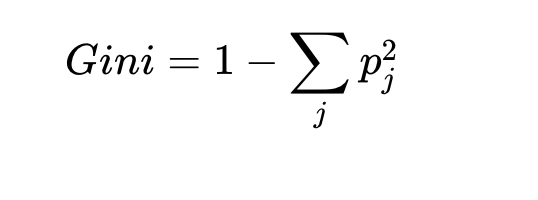
\includegraphics{Screen Shot 2018-06-28 at 10.53.42 PM.png}
\caption{alt text}
\end{figure}

\begin{verbatim}
b. Gini Split

    ??

c. Entropy
    
    Entropy is a measure for (un-)orderedness
    
\end{verbatim}

\begin{figure}
\centering

\includegraphics{Screen Shot 2018-06-28 at 10.59.28 PM.png}
\caption{alt text}
\end{figure}

\begin{verbatim}
d. Gain Split

    ??
    
e. Gain Ratio

    modification of the information gain that reduces its bias towards multi-valued attributes_
    
f. Misclassification Rate

    ??
\end{verbatim}

    \paragraph{4. Consider the following training set for a binary
classification problem to predict whether a customer is likely to renew
the subscription to a certain magazine based on gender and car
type:}\label{consider-the-following-training-set-for-a-binary-classification-problem-to-predict-whether-a-customer-is-likely-to-renew-the-subscription-to-a-certain-magazine-based-on-gender-and-car-type}

\begin{verbatim}
a. Create subsamples based on Gender and compute the percentage of Yes and No in each split. Fill the following tables

| Renew         | Y             | N     |
| ------------- | ------------- | ----- |
| Gender=M      | 60%           | 40%   |

| Renew         | Y             | N     |
| ------------- | ------------- | ----- |
| Gender=F      | 28%           | 42%   |

b. Create subsamples based on Car type and compute the percentage of Yes and No in each split. Fill the following tables

| Renew         | Y             | N     |
| ------------- | ------------- | ----- |
| CarType=F     | 50%           | 50%   |

| Renew         | Y             | N     |
| ------------- | ------------- | ----- |
| CarType=L     |  10%           | 90%  |


| Renew         | Y             | N     |
| ------------- | ------------- | ----- |
| CarType=L     |  100%         | 0%    |


c. Which attribute creates the best split in terms of purity of subsamples? There is no need to provide exact values for information gain. Just compare distribution of Y/N.

CarType=L 

d. Compute the Entropy and Gini Index of “Gender”, “CarType”, and “Renew”.

??

e. Select the “best” splitting attribute based on Gain Split, and build the first branch of the tree. Then use the other attributes to split the subsamples further.

??
\end{verbatim}


    % Add a bibliography block to the postdoc
    
    
    
    \end{document}
